% !TeX document-id = {88ddee8b-8eb6-46e0-9af4-2c10d8b61c04}
% !TeX spellcheck = de-DE
% !TeX encoding = utf8
% !TeX TXS-program:compile = txs:///pdflatex/[--shell-escape]

% This is LLNCS.DEM the demonstration file of
% the LaTeX macro package from Springer-Verlag
\documentclass[a4paper,12pt]{llncs}
%
\usepackage{makeidx}  % allows for indexgeneration
\makeindex

\usepackage[ngerman]{babel}
\usepackage[utf8]{inputenc}      % Code-Page latin 1
\usepackage[T1]{fontenc}
% Nur eine der beiden folgenden Zeilen einbinden!
% siehe Abschnitt Bilder
%\usepackage{graphicx}       % Bilder einbinden, Version fuer normales latex
\usepackage[pdftex]{graphicx}       % Bilder einbinden, Version fuer pdflatex

% mit Hyperrefs
\usepackage[pdftex, plainpages=false,hypertexnames=true,pdfnewwindow=true,backref=true,colorlinks=true,citecolor=blue,linkcolor=black,urlcolor=blue,filecolor=blue]{hyperref}% 
% weitere Packages
\usepackage{ifthen}                 % Zum Auskommentieren von Textteilen
\usepackage{amssymb}                % Mathematische Buchstaben
\usepackage{amsmath}                % Verbesserter Formelsatz
%\usepackage[vlined,boxed]{algorithm2e}
\usepackage{booktabs}               % schönere Tabellen
\usepackage{color}
\usepackage{algpseudocode}			% Für Pseudocode Algorithmen
\usepackage{tcolorbox}
\usepackage{hyperref}
 \hypersetup{urlcolor=black,citecolor=black}

%\setalcapskip{1.5ex} % fuer package algorithm
\usepackage{dsfont}  
%\newtheorem{definition}{Definition}
\usepackage{doc}
\usepackage{mathrsfs}
\usepackage{mathtools}
\usepackage{todonotes}
\usepackage{subfigure}

% Seitenformat ===============================================================
\hoffset=-1.25truecm
\setlength{\topmargin}{0.0cm}
\setlength{\textheight}{23.0cm}
\setlength{\footskip}{1.5cm}
\setlength{\textwidth}{15.4cm}
\setlength{\evensidemargin}{1.5cm}
\setlength{\oddsidemargin}{1.5cm}
\setlength{\parskip}{1ex}
\setlength{\parindent}{0pt}
\setlength{\marginparwidth}{1.4cm}
\setlength{\marginparsep}{1mm}

\pagestyle{plain}

% Makro-Definitionen ==========================================================

% 
\def\myverzeichnis{.}

\numberwithin{equation}{section} 
% Bild -----------------------------------------------------------------------
% #1 Filename;  #2 Label;  #3 Bildunterschrift;  #4 Kurzform
\newcommand{\bild}[4]{
  \begin{figure}[htbp]
    \begin{center}
      \includegraphics{#1}
      \caption[#4]{#3}
      \label{#2}
    \end{center}
  \end{figure}
}

% Bildbreite -----------------------------------------------------------------
% #1 Filename;  #2 Breite;  #3 Label;  #4 Bildunterschrift;  #5 Kurzform
\newcommand{\bildbreite}[5]{
  \begin{figure}[htbp]
    \begin{center}
      \includegraphics[width=#2]{#1}
      \caption[#5]{#4}
      \label{#3}
    \end{center}
  \end{figure}
}

\newtheorem{satz}{Satz}
\newtheorem{korollar}{Korollar}

\DeclareMathOperator{\hit}{hit}
\DeclareMathOperator{\shot_count}{shot\_count}
\DeclareMathOperator{\strat}{strat}
\DeclareMathOperator{\strategies}{strategies}
\DeclareMathOperator{\sunk}{sunk}


% ============================================================================
\begin{document}

% =========== Das war der Vorspann, jetzt geht's los! ========================

% ============================================================================
% =============  AB HIER DARF UND SOLL GETIPPT WERDEN ========================
% ============================================================================
\author{Viel Schreiber}
\index{Viel Schreiber}

% Das Institut wird fuer den Betreuer missbraucht ...
\institute{{\bf Betreuer:} Dipl.-Inf. Carl Coder}
\authorrunning{Viel Schreiber}
\title{Meine Seminarausarbeitung}

\maketitle

%\todo[inline]{Version \gitAbbrevHash, Branch \gitBranch, \gitCommitterIsoDate \gitDirty}

\thispagestyle{empty}

\begin{abstract}
Ein schöner Abstract. Das ist einfach die Kurzzusammenfassung.
\end{abstract}

% Einleitung -----------------------------------------------------------------
\section{Einleitung}

\subsection{Spielbeschreibung}
\nocite{WB95} % Mindestens eine Zitierung ist nötig, damit BibTex funktioniert
Diese Ausarbeitung beschäftigt sich mit der Umsetzung von Schiffe-Versenken in beliebig viele Dimensionen.
Die generelle Funktionsweise von dem normalen Schiffe-Versenken bleibt erhalten, muss jedoch um einige Dinge erweitert werden, um auch in höheren Dimensionen gut spielbar zu sein.

Zu Beginn platziert der Gegner eine beliebige Anzahl an Schiffen auf seinem Spielfeld. Es wird davon ausgegangen, dass die Schiffspositionen rein zufällig ausgewählt wurden, d.h. dass zu Spielbeginn eine Flotte aus der Menge aller möglichen Flotten ausgewählt wird. Jede mögliche Flotte hat hierbei die gleiche Wahrscheinlichkeit, ausgewählt zu werden.
Natürlich sind die Schiffspositionen dem Spieler nicht bekannt.
Die Gesamtheit aller gewählten Schiffspositionen wird auch die Flotte genannt.
Nun kann der Spieler anfangen, auf bestimmte Positionen auf dem Spielfeld, auch Zellen genannt, zu schießen.
Da Schiffe überlappen können, können mit jedem Schuss mehrere Schiffe, also Teilmengen der Flotte getroffen werden.
Nach jedem Schuss erfährt der Spieler von seinem Gegner, welche Teilmenge der Flotte er getroffenen hat.
Falls keine Schiffe getroffen wurden ist diese Menge natürlich leer.
Ein Schiff gilt als versenkt, sobald es getroffen wurde.
Sobald alle Schiffe versenkt wurden, ist das Spiel beendet.
Das Ziel des Spielers ist es, mit möglichst wenig Schüssen alle Schiffe zu versenken.

\subsection{Inhalt der Ausarbeitung}

Der erste Teil dieser Ausarbeitung beschäftigt sich mit der Bewertung einer gegebenen Strategie, d.h. mit der Berechnung der erwarteten Anzahl an Schüssen, die mit einer Strategie zum versenken der platzierten Flotte gebraucht werden.
Da diese Berechnung sehr aufwändig ist, wird ein Monte-Carlo Algorithmus zur näherungsweisen Berechnung beschrieben, implementiert und ausgewertet.

Im zweiten Teil werden unter den zuvor etablierten Rahmenbedingungen verschiedene Strategien vorgestellt. Dabei können sich diese von denen in der Bachelorarbeit vorgestellten unterschieden, da es sich um andere Rahmenbedingungen handelt. Zu den Strategien zählen dünne und volle Gitter, klassisches und Quasi Monte Carlo und die optimale Maximum Strategie.

Dritter Teil (Implementierung + Vergleich) TODO 

\section{Formalisierung des Spielprinzips}

\begin{definition}
Sei
\[
C_{all} \coloneqq \{1, \dots, N\}^d
\]
die Menge aller Zellen des Spielfeldes mit jeweils $N$ Zellen in $d$ Dimensionen.
\end{definition}

\begin{satz}
Dann gilt:
\[
|C_{all}|=N^d
\]
\end{satz}

\begin{definition}
Seien $c, c' \in C_{all}$ Zellen.
Dann ist
\[
c \leq c' \Leftrightarrow \forall i \in \{1, \dots, d\} \colon c_{i} \leq c'_{i} 
\]
\end{definition}

\begin{definition}
Sei $c_{min} \in C_{all}$ und $c_{max} \in C_{all}$ mit $c_{min} \leq c_{max}$.
\[
l=(c_{min}, c_{max})
\]
eine mögliche Schiffsposition (location), welche mithilfe einer minimalen Ecke $c_{min}$ und einer maximalen Ecke $c_{max}$ bestimmt wird.
\end{definition}

\begin{definition}
Sei 
\[
L_{all} \coloneqq
\{
(i, j) \in C_{all} \times C_{all}
\mid
i \leq j
\}
\] die Menge aller möglichen Schiffspositionen.
\end{definition}

\begin{satz}
Dann gilt:
\[
|L_{all}|=\left(\frac{(N+1) N}{2}\right)^d
\]
\end{satz}

\begin{proof}
Da das Spielfeld in jeder Dimension die Größe $N$ hat, gilt in jeder Dimension $d$ für gültige Start- und Endkoordinaten eines Schiffes $c_d$ und $c'_d$ mit $c_d \leq c'_d$ folgendes:
\begin{align}
\begin{split}
&|\{(c_d, c'_d) \in N \times N \mid c_d \leq c'_d\}|\\
&=|\{(i, j) \in N \times N \mid i \leq j\}|\\
&=\sum_{i=1}^N N - i + 1\\
&=N + \sum_{i=1}^{N-1} i\\
&=\sum_{i=1}^{N} i\\
&= \frac{(N + 1) N}{2}
\nonumber
\end{split}
\end{align}
Daher gibt es genau
\[
\left(\frac{(N+1) N}{2}\right)^d
\]
gültige Schiffspositionen, da für jede Schiffsposition für jede Dimension gültige Start- und Endkoordinaten gewählt werden müssen, also genau $d$ gültige Start- und Endkoordinaten.
\end{proof}

\begin{definition}
Sei 
\[
K \coloneqq \{1, \dots, |L_{all}|\}
\]
die Menge aller möglichen Flottengrößen.
\end{definition}

\begin{definition}
Sei $k \in K$ die Größe der Flotte.
Dann ist
\[
F_{all,k} \coloneqq\{F \in \mathcal{P}(L_{all}) \mid |F| = k\}
\]
die Menge aller Flotten der Größe $k$.
\end{definition}

\begin{satz}
Sei $k \in K$ die Größe der Flotte.
Dann gilt:
\[
|F_{all,k}|=\binom{|L_{all}|}{k}
\]
\end{satz}

\begin{definition}
Dann ist
\[
F_{all} \coloneqq \bigcup_{k=1}^{|L_{all}|} F_{all,k} = \mathcal{P}(L_{all}) \setminus \{\emptyset\}
\]
\end{definition}

\begin{satz}
Dann gilt:
\[
|F_{all}|=2^{|L_{all}|} - 1
\]
\end{satz}

\begin{proof}
\begin{align}
\begin{split}
&|F_{all}|=\sum_{k=1}^{|L_{all}|} |F_{all,k}|\\
=&\sum_{k=1}^{|L_{all}|} \binom{|L_{all}|}{k} \\
=&\left( \sum_{k=0}^{|L_{all}|} \binom{|L_{all}|}{k} \right) - 1 \\
=&2^{|L_{all}|} - 1
\end{split}
\end{align}
\qed
\end{proof}


\begin{definition}
Sei $F \in F_{all}$ und $c \in C_{all}$.
Dann ist 
\begin{align}
&\hit:F_{all} \times C_{all} \rightarrow \mathcal{P}(L_{all}) \quad mit \nonumber\\
&\hit(F, c)\mapsto \{(c_{min}, c_{max}) \in F \mid c_{min} \leq c \leq c_{max}\} \nonumber
\end{align}
die Treffer-Funktion, welche angibt, welche Schiffe bei einem Schuss auf Zelle $c$ getroffen wurden, falls $F$ die vom Gegner platzierte Flotte ist. In anderen Worten, die Menge der Schiffe aus Flotte $F$, die die Zelle $c$ belegen.
\end{definition}

\subsection{Schuss-Strategien}

\begin{definition}
Eine Funktion der Form
\begin{align}
&\strat:\mathcal{P}(C_{all}) \rightarrow C_{all} \nonumber
\end{align}
wird Strategiefunktion genannt. Diese wählt die nächste Zelle aus, auf die geschossen werden soll, abhängig davon, auf welche Zellen bereits geschossen wurden.
\end{definition}

\begin{definition}
Sei
\[
\strategies  \coloneqq \{ \strat:P(C_{all}) \rightarrow C_{all} \}
\]
die Menge an allen Strategiefunktionen.
\end{definition}

\begin{definition}
Sei $F\in F_{all}$ die gewählte Flotte und $S \in P(C_{all})$ die Menge an bereits beschossenen Zellen.
Dann ist:
\[
\sunk(F, S) \Leftrightarrow \bigcup_{c \in S} \hit(F, c) = F
\]
wahr, falls alle Schiffe aus der Flotte $F$ versenkt wurden.
\end{definition}


\begin{definition}
Sei $F\in F_{all}$ die gewählte Flotte und $S$ die Menge an bereits beschossenen Zellen.
Sei außerdem $\strat \in \strategies$ die verwendete Schuss-Strategie.
Dann ist
\begin{align}
&\shot_count(F, S, \strat)=
& \begin{cases} 
  	0& ,\sunk(F, S) \\
      \shot_count(F, S \cup \strat(S), \strat) + 1 & ,sonst
   \end{cases}
\nonumber
\end{align}
die Anzahl an Schüssen, die benötigt werden, um alle Schiffe der Flotte $F$ mit der Schuss-Strategiefunktion $\strat$ zu versenken, falls bereits auf die Zellen der Menge $S$ geschossen wurde.

Außerdem ist dann
\begin{align}
&\shot_count(F, \strat)=\shot_count(F, \emptyset, \strat)
\nonumber
\end{align}
die Anzahl an Schüssen, die benötigt werden, um alle Schiffe der Flotte $F$ mit der Schuss-Strategiefunktion $\strat$ zu versenken.
\end{definition}

\subsection{Zufallsvariablen}

\begin{definition}
Sei $\Omega \subseteq F_{all}$ eine Menge an Flotten.
\end{definition}

\begin{definition}
Sei $A \subseteq \Omega$ das Ereignis, dass bei einem Auswählen einer Flotte aus $\Omega$, die Flotte ebenfalls in der Menge $A$ liegt.
Dann ist
\[
P(A) = \frac{|A|}{|\Omega|}
\]
die Wahrscheinlichkeit, dass eine Flotte aus der Menge $A$ ausgewählt wird.
\end{definition}

Dann ist $(\Omega, P)$ ein endlicher Laplacescher W-Raum und P eine Gleichverteilung.

\begin{definition}
Sei $\strat \in \strategies$ die verwendete Schuss-Strategie.
Sei $\omega$ die ausgewählte Flotte aus $\Omega$.
Dann ist
\begin{align}
\mathbf{T}_{\strat}(\omega) \coloneqq \shot_count(\omega, \strat)
\nonumber
\end{align}
eine Zufallsvariable, die die Anzahl an Schüssen zum versenken einer Flotte $\omega$ bezeichnet.
\end{definition}

\begin{satz}
Sei $\strat \in \strategies$ die verwendete Schuss-Strategie.
Dann ist
\begin{align}
E_\Omega(\mathbf{T}_{\strat})=\frac{1}{|\Omega|} \sum_{\omega \in \Omega} \shot_count(\omega, \strat)
\nonumber
\end{align}
der Erwartungswert von $\mathbf{T}_{\strat}$ in der Menge $\Omega$.
\end{satz}

\begin{proof}
\begin{align}
\begin{split}
E_\Omega(\mathbf{T}_{\strat})&=\sum_{\omega \in \Omega} P(\omega) \shot_count(\omega, \strat)\\
&=\frac{1}{|\Omega|} \sum_{\omega \in \Omega} \shot_count(\omega, \strat)
\nonumber
\end{split}
\end{align}
\qed
\end{proof}

\begin{satz}
Sei $\strat \in \strategies$ die verwendete Schuss-Strategie.
Dann ist
\begin{align}
E_{F_{all}}(\mathbf{T}_{\strat})=\frac{1}{|F_{all}|} \sum_{k=1}^{|L_{all}|}\sum_{F\in F_{all,k}} \shot_count(F, \strat)
\nonumber
\end{align}
der Erwartungswert von $\mathbf{T}_{\strat}$ in der Menge $F_{all}$.
\end{satz}

\begin{proof}
\begin{align}
\begin{split}
&E_{F_{all}}(\mathbf{T}_{\strat})\\
=&\frac{1}{|F_{all}|} \sum_{F\in F_{all}} \shot_count(F, \strat)\\
=&\frac{1}{|F_{all}|} \sum_{k=1}^{|L_{all}|}\sum_{F\in F_{all,k}} \shot_count(F, \strat)
\nonumber
\end{split}
\end{align}
\qed
\end{proof}

\begin{definition}
Sei $k \in K$ die Flottengröße.
Dann ist
\[
g_k=\frac{|F_{all,k}|}{|F_{all}|}=\frac{\binom{|L_{all}|}{k}}{2^{|L_{all}|} - 1}
\]
der Anteil an Flotten der Größe $k$ an der Menge aller Flotten. Dieser Faktor wird später als Gewichtungsfaktor für den Erwartungswert der Flottengröße $k$ verwendet.
\end{definition}

\begin{satz}
Sei $\strat \in \strategies$ die verwendete Schuss-Strategie.
Dann ist
\begin{align}
E_{F_{all}}(\mathbf{T}_{\strat})=\sum_{k=1}^{|L_{all}|} g_k E_{F_{all,k}}(\mathbf{T}_{\strat})
\nonumber
\end{align}
der Erwartungswert von $\mathbf{T}_{\strat}$ in der Menge $F_{all}$.
\end{satz}

\begin{proof}
\begin{align}
\begin{split}
&E_{F_{all}}(\mathbf{T}_{\strat})\\
=&\frac{1}{|F_{all}|} \sum_{k=1}^{|L_{all}|}\sum_{F\in F_{all,k}} \shot_count(F, \strat)\\
=&\sum_{k=1}^{|L_{all}|} \frac{1}{|F_{all}|} \sum_{F\in F_{all,k}} \shot_count(F, \strat)\\
=&\sum_{k=1}^{|L_{all}|} \frac{1}{|F_{all}|} |F_{all,k}| \sum_{F\in F_{all,k}} \frac{1}{|F_{all,k}|} \shot_count(F, \strat)\\
=&\sum_{k=1}^{|L_{all}|} \frac{|F_{all,k}|}{|F_{all}|} E_{F_{all,k}}(\mathbf{T}_{\strat})\\
=&\sum_{k=1}^{|L_{all}|} g_k E_{F_{all,k}}(\mathbf{T}_{\strat})
\nonumber
\end{split}
\end{align}
\qed
\end{proof}

\section{Berechnung des Erwartungswertes mithilfe eines MC-Algorithmus}

Um zu bewerten, wie gut eine Strategiefunktion $\strat$ abschneidet, kann ein Monte-Carlo Algorithmus implementiert werden, der für jede Flottengröße $k \in K$ mit einer Stichprobe den Wert von $E_{F_{all,k}}(\mathbf{T}_{\strat})$ abschätzt und am Ende alle diese Werte zum gesamtem Erwartungswert $E_{F_{all}}(\mathbf{T}_{\strat})$ kombiniert.

Um den Wert von $\shot_count(F, \strat)$ für eine gegebene Flotte $F$ zu berechnen, kann folgende, (naive) Funktion verwendet werden:

\begin{tcolorbox}
	\begin{algorithmic}[H]
		\Function{shot\_count}{$F, \strat$}{:}
		\State $S=\emptyset$;
		\State $\shot_count=0$;
		\While{$\neg \sunk(F, S)$}
		\State $next\_target=\strat(S)$;
		\State $S=S \cup \hit(F, next\_target)$;
		\State $\shot_count=\shot_count+1$;
		\EndWhile
		\State\Return $\shot_count$;
		\EndFunction
	\end{algorithmic}
\end{tcolorbox}

Um damit dann einen kompletten Algorithmus implementieren zu können, muss jedoch erst eine Abbruchbedingung formuliert werden, die bestimmt, wann für eine Flottengröße $k \in K$ der approximierte Wert von $E_{F_{all,k}}(\mathbf{T}_{\strat})$ gut genug ist.

Dafür ist es nützlich, die Erwartungswertänderung wie in dem folgenden Satz darzustellen:

\begin{satz}
Sei $G_k^{(n)} \subseteq F_{all,k}$ eine Teilmenge der Flotten mit Größe $k$ mit $|G_k^{(n)}|=n$.
Sei außerdem $F_k^{(n+1)} \in (F_{all,k} \setminus G_k^{(n)})$ eine weitere, noch nicht ausgewertete Flotte.
Dann ist $G_k^{(n+1)}=G_k^{(n)} \cup F_k^{(n+1)}$ und für den Erwartungswert gilt:
\begin{align}
E_{G_k^{(n+1)}}(\mathbf{T}_{\strat})=E_{G_k^{(n)}}(\mathbf{T}_{\strat}) + \delta\\
 \delta=\frac{\mathbf{T}_{\strat}(F_k^{(n+1)}) - E_{G_k^{(n)}}(\mathbf{T}_{\strat})}{n+1}
\nonumber
\end{align}
\end{satz}

\begin{proof}
Sei
\begin{align}
\begin{split}
s=\sum_{F \in G_k^{(n)}} \mathbf{T}_{\strat}(F),\;\; E_{G_k^{(n)}}(\mathbf{T}_{\strat}) =\frac{s}{n}
\end{split}
\end{align}
Dann ist
\begin{align}
\begin{split}
&E_{G_k^{(n+1)}}(\mathbf{T}_{\strat})\\
=&\frac{s+ \mathbf{T}_{\strat}(F_k^{(n+1)}) }{n + 1}\\
=&\frac{s}{n + 1} + \frac{\mathbf{T}_{\strat}(F_k^{(n+1)}) }{n + 1}\\
=&\frac{s}{n} * \frac{n}{n + 1} + \frac{\mathbf{T}_{\strat}(F_k^{(n+1)}) }{n + 1}\\
=&E_{G_k^{(n)}}(\mathbf{T}_{\strat}) * (1 - \frac{1}{n + 1}) + \frac{\mathbf{T}_{\strat}(F_k^{(n+1)}) }{n + 1}\\
=&E_{G_k^{(n)}}(\mathbf{T}_{\strat}) - \frac{E_{G_k^{(n)}}(\mathbf{T}_{\strat})}{n + 1}) + \frac{\mathbf{T}_{\strat}(F_k^{(n+1)}) }{n + 1}\\
=&E_{G_k^{(n)}}(\mathbf{T}_{\strat}) + \frac{E_{G_k^{(n)}}(\mathbf{T}_{\strat}) - \mathbf{T}_{\strat}(F_k^{(n+1)}) }{n + 1}\\
\end{split}
\end{align}
\qed
\end{proof}

Damit kann dann eine Abbruchbedingung formuliert werden, die angibt, wie groß die Flottenanzahl $n$ sein muss, damit Veränderung des Erwartungswertes $\delta$ für eine zusätzlich ausgewertete Flotte $F_k^{(n+1)}$ einen Grenzwert $\delta_{min}$ immer unterschreitet:

\begin{satz}
Sei $\delta_{min} > 0$.
Dann gilt:

\begin{align}
n = \left\lceil \frac{|C_{all}| - 1}{\delta_{min}} \right\rceil - 1 \Rightarrow |\delta| \leq \delta_{min}
\nonumber
\end{align}
\end{satz}

\begin{proof}
\begin{align}
|\delta|=\frac{|\mathbf{T}_{\strat}(F_k^{(n+1)}) - E_{G_k^{(n)}}(\mathbf{T}_{\strat})|}{n+1} \leq \delta_{min}\\
\Leftrightarrow \frac{|\mathbf{T}_{\strat}(F_k^{(n+1)}) - E_{G_k^{(n)}}(\mathbf{T}_{\strat})|}{\delta_{min}} \leq (n+1)
\nonumber
\end{align}
Da $\forall F \in F_{all} \colon \mathbf{T}_{\strat}(F) \leq |C_{all}|$ und $\forall G \subseteq F_{all} \colon E_{G}(\mathbf{T}_{\strat}) \geq 1$ gilt:
\begin{align}
\begin{split}
\left( (n+1) \geq \frac{|C_{all}| - 1}{\delta_{min}} \Rightarrow |\delta| \leq \delta_{min} \right)\\
\Rightarrow \left(n = \left\lceil \frac{|C_{all}| - 1}{\delta_{min}} \right\rceil - 1 \Rightarrow |\delta| \leq \delta_{min} \right)
\end{split}
\end{align}
\qed
\end{proof}

Diese Abschätzung ist sehr großzugüg gewählt. Es wird sehr oft passieren, dass bereits für kleinere Werte von $n$ der Grenzwert $\delta_{min}$ unterschritten wird, jedoch kann mit dieser größeren Wahl von $n$ garantiert werden, dass der Grenzwert $\delta_{min}$ in jedem zusätzlichen Schritt unterschritten wird. Daher muss nicht nach jedem Schritt eine Abbruchbedingung überprüft werden, sondern nur zu Beginn die Anzahl der Schritte $n$ einmalig berechnet werden.

\begin{tcolorbox}
	\begin{algorithmic}[H]
		\Function{simulate\_rounds}{$k, \strat, \delta_{min}$}{:}
		\State $n =\left\lceil \frac{|C_{all}| - 1}{\delta_{min}} \right\rceil - 1$;
		\State //Generiere $n$ verschiedene Flotten der Größe $k$;
		\State $fleets = generate\_random\_fleets(k, n)$;
		\State $sum=0$;
		\For{$i=1,\dots,n$}
		\State $sum += shot\_count(fleets[i], \strat)$;
		\EndFor
		\State\Return $\frac{sum}{n}$;
		\EndFunction
	\end{algorithmic}
\end{tcolorbox}


Abschliessend kann dann die Funktion implementiert werden, die den Wert von $E_{F_{all}}(\mathbf{T}_{\strat})$ für Flotten beliebiger Größe berechnet. Dafür müssen die berechneten Werte von $E_{F_{all,k}}(\mathbf{T}_{\strat})$ für jedes $k$ gewichtet aufsummiert werden. Nebenbei werden auch die Erwartungswerte für jedes $k$ gespeichert, damit diese später auch untersucht werden können.

\begin{tcolorbox}
\begin{algorithmic}[H]
	\Function{calculate\_expected\_shot\_count}{strat, $\epsilon, \eta$}{:}
	\State $expected\_shot\_count=[]$;
	\State $total\_expected\_shot\_count=0$;
	\For{$k=1$ to $|L_{all}|$}
	\State $g_k=\frac{|F_{all,k}|}{|F_{all}|}$;
	\State $\delta_k=g_k * \delta$;
	\State $E=simulate\_rounds(k, strat, \delta_k)$;
	\State $expected\_shot\_count[k] = E$;
	\State $total\_expected\_shot\_count+=g_k * E$;
	\EndFor
	\EndFunction
\end{algorithmic}
\end{tcolorbox}


\section{Strategien}

Der folgende Abschnitt befasst sich mit Schussstrategien. In \cite{M13} wurden diskrepanzminimierende Diskretisierungsverfahren erstmals als potentielle Schussstrategien eingeführt. Dabei wurden die von diesen Verfahren genutzten Stützstellen meist als Schussfolgen interpretiert. Zu Beginn wird noch einmal die optimale Strategie aus \cite{M13} aufgegriffen um diese in der hier eingeführten Notation darzustellen, da sich die Rahmenbedingungen dieser Ausarbeitung doch von \cite{M13} unterscheiden. Anschließend werden noch andere Strategien, wie dünne und volle Gitter, klassisches und Quasi Monte-Carlo betrachtet. 

Sei für alle folgenden Strategien $F\in F_{all}$ die aktuell vorliegende unbekannte Flotte.

\subsection{Maximum Strategie}

Diese in \cite{M13} Abbildung 3.15 vorgestellte Strategie berechnet zunächst eine Anfangsverteilung. Dabei wird für jeden Punkt im betrachteten $d$-dimensionalen Raum festgestellt wie viele Schiffe diesen Punkt enthalten. Anschließend wird dem Punkt diese Anzahl zugewiesen. Von diesen Punkten wird dann das Maximum bezüglich dieser Anzahl bestimmt. Das ist dann die Zelle auf die als nächstes geschossen wird.

In \cite{M13} wurden alle möglichen Schiffspositionen auf einmal betrachtet und von diesen Verteilungen die Maxima berechnet. Allerdings betrachten wir in dieser Ausarbeitung nur verschiedene unbekannte Flotte $F$ in mehreren Experimenten. Daraus versuchen wir dann im Monte-Carlo Prinzip eine allgemeine Aussage für alle Flotten abzuleiten. Das heißt in diesem Fall wird das Maximum an einer anderen Stelle berechnet als noch in \cite{M13}. 

Der Algorithmus für die Maximum bzw. optimale Strategie sieht dann folgendermaßen aus:

\begin{tcolorbox}
	\begin{algorithmic}
		\Function{max\_strat}{$S$}{$:cell$}
		\State $cell = null$;
		\State $max = 0$;
		\State $temp = 0$;
		\For{\textbf{each } $c\in C_{all}$}
		\State $temp=\left|\hit(F,c)\right|$;
		\If{$temp>max$}
		\State $max=temp$;
		\State $cell = c$;
		\EndIf
		\EndFor
		\State \Return $cell$;
		\EndFunction
	\end{algorithmic}
\end{tcolorbox}

Wie in \cite{M13} ebenfalls angesprochen hat diese Art der Herangehensweise ganz unabhängig von den Rahmenbedingungen horrende Kosten. Wir wollen hier erst einmal nur die Kosten eines Strategieaufrufs betrachten. Dabei wird über alle Zellen des Spielfelds iteriert, das heißt wir haben $N^d$ Schleifendurchläufe pro Aufruf der Strategie. In jedem dieser Durchläufe wird die $\hit$ Funktion aufgerufen. Diese muss für jedes Schiff aus der aktuellen Flotte $F$ prüfen ob dieses die momentan anvisierte Zelle $c$ enthält. Diese Überprüfung kann mittels zwei arithmetischen Vergleichen (Erinnerung: ein Schiff wird als Tupel $(c_{min},c_{max})$ gespeichert) erledigt werden. Damit haben wir für den Aufruf der $\hit$ Funktion Kosten von $O(2\cdot |F|)$, bzw. wenn wir gleich den Betrag hinzunehmen $O(3\cdot |F|)$. Zusammengefasst befinden wir uns also bei einem Aufruf der Maximumsstrategie bei Kosten von $O(N^d\cdot3|F|)$. Damit ist diese Strategie für eine Realisierung in hohen Dimensionen zu teuer. 

\subsection{Gitter Strategien}

In Abschnitt 2.2.1 von \cite{M13} werden die hierarchischen Stützstelleninkremente $H_{\underline{m}}$ für Gitter vorgestellt, welche sich von den in \cite{M13} Abbildung 2.2 dargestellten Hütchenfunktionen ableiten. Diese Inkremente bzw. ihre Kombinationen werden sowohl für dünne als auch volle Gitter genutzt. Dabei halbiert sich die Maschenweite mit steigendem Level in einer beliebigen Dimension. Dies ist schön zu sehen in Abbildung \ref{fig:gitter01} (Vgl. \cite{P10} Figure 2.5). Hier liegen die Stützstellen höherer Level zwischen den Linien, die durch ihre Vorgänger entstanden sind.

Es lassen sich durch Kombinationen von Inkrementen Gitter erzeugen. Unsere Schussfolge ergibt sich dann aus den abgearbeiteten Inkrementen bzw. den darin enthaltenen Stützstellen. 

\begin{figure}
	\centering
	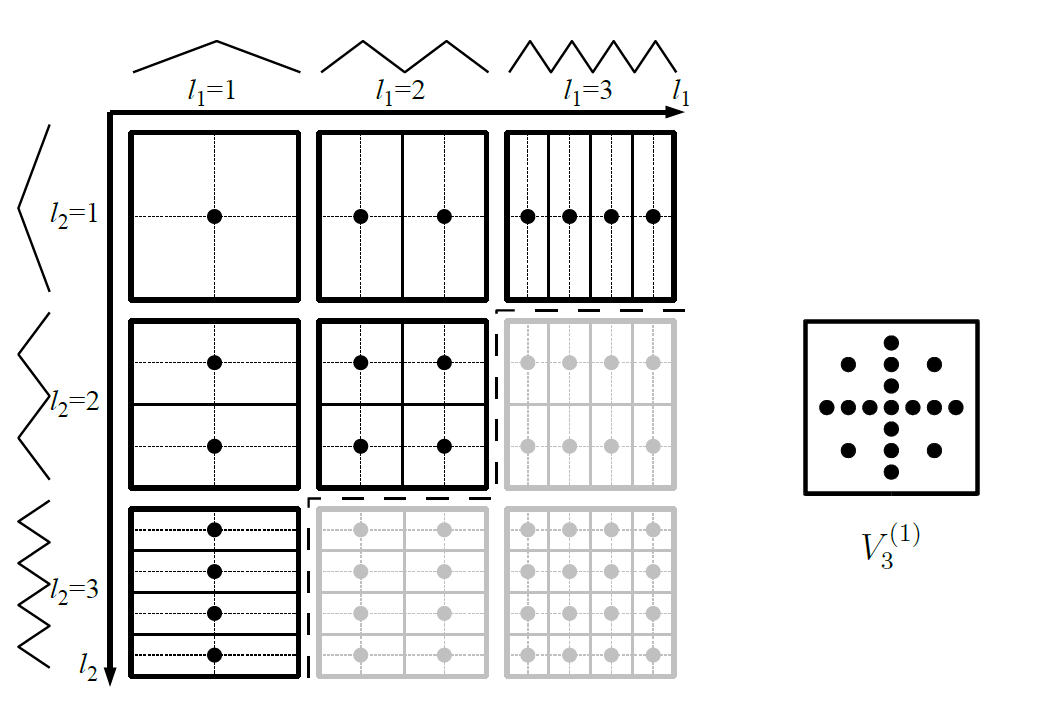
\includegraphics[width=0.75\linewidth]{figures/Gitter01}
	\caption{Kopie zur Verdeutlichung von \cite{P10} Figure 2.5}
	\label{fig:gitter01}
\end{figure}


Noch zu beachten ist, dass es bei Gittern so genannte Level gibt, die die Maschenweite und damit die Genauigkeit angeben. Normalerweise legt man ein Level fest und erzeugt sich dann aus Inkrementen ein Gitter eben dieses Levels. In unseren Fall arbeiten wir uns durch die Inkremente bei steigendem Level aufsteigend durch um immer genauere Gitter zu erzeugen, bis wir alle Schiffe der Flotte getroffen haben.

\subsubsection{Volle Gitter Strategie}

In \cite{M13} Definition 2.14 wird beschrieben, wie sich volle Gitter aus den Inkrementen zusammensetzen. Dabei ist lediglich zu beachten, dass die Indeces eines Inkrements $H_{\underline{m}}$ nur kleiner dem Level $n$ sein müssen.  Zur Wiederholung:

\begin{definition}
	Seien $d,n\in\mathbb{N}$ und $d,n>1$. Ein $d$-dimensionales volles Gitter $G$ mit Level $n$ wird durch Kombination der Inkremente $H_{\underline{m}}$ mit $\underline{m}<(n,\dots,n)$ erzeugt:
	\begin{equation}
		G=\biguplus_{m_1=1}^n\biguplus_{m_2=1}^n\dots \biguplus_{m_d=1}^n H_{\underline{m}}
	\end{equation}
\end{definition}

Diese Definition kann anhand Abbildung \ref{fig:gitter02} verdeutlicht werden. Darin sind einige mögliche Kombinationen von Inkrementen markiert, die ein volles Gitter von Level 2 bis 4 bilden.

\begin{figure}
	\subfigure[Volles Gitter Level 2]{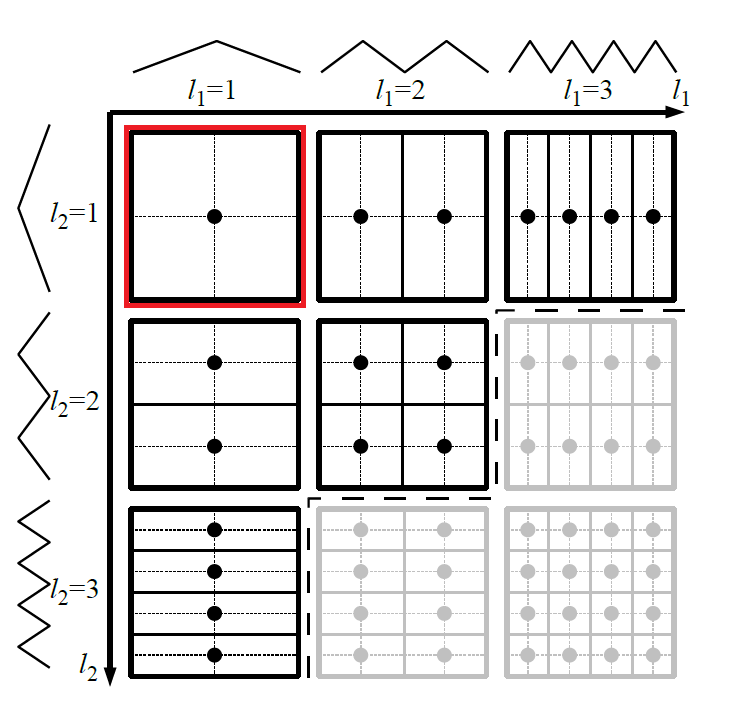
\includegraphics[width=0.30\textwidth]{figures/Gitter02}}
	\subfigure[Volles Gitter Level 3]{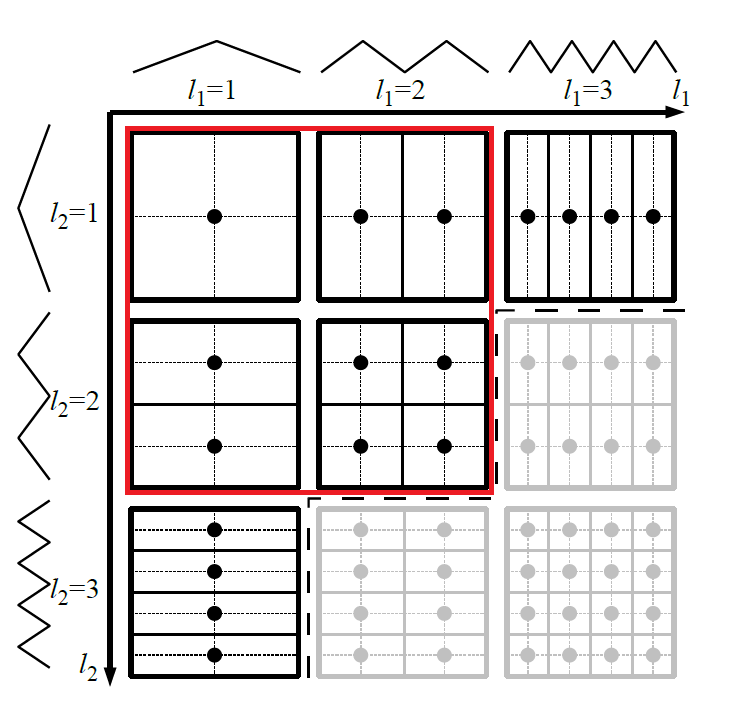
\includegraphics[width=0.30\textwidth]{figures/Gitter03}}
	\subfigure[Volles Gitter Level 4]{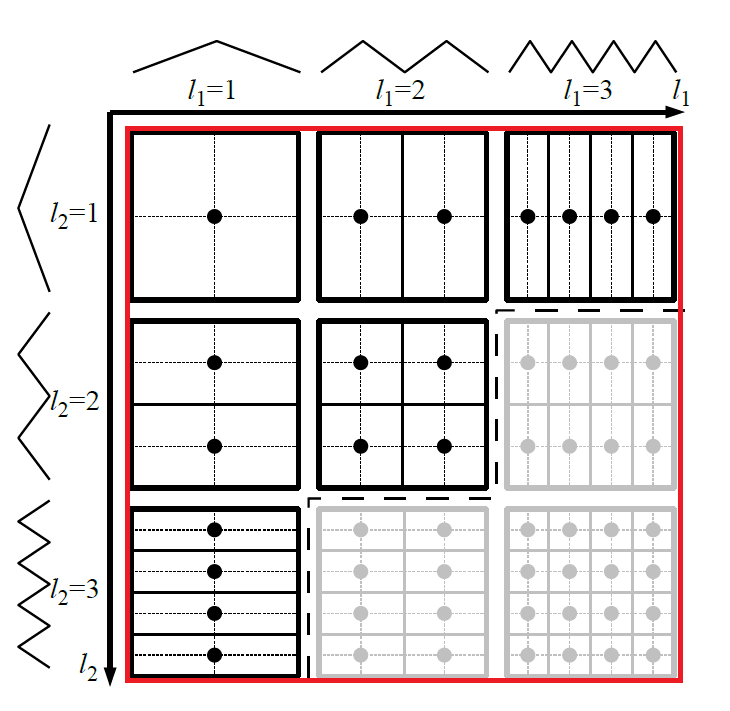
\includegraphics[width=0.30\textwidth]{figures/Gitter04}}
	\caption{Beispiele für zweidimensionale volle Gitter}
	\label{fig:gitter02}
\end{figure}

Wie man gut an Abbildung \ref{fig:gitter02} sehen kann können volle Gitter kleineren Levels für größere genutzt werden. Wenn man also eine Schussfolge abarbeiten möchte, die immer genauer wird kann man zunächst mit einem vollen Gitter Level 2 starten und dann lediglich die neu hinzukommenden Inkremente abarbeiten. Das heißt beim Iterieren können wir uns an den Levels orientieren.

Wir können an Abbildung \ref{fig:gitter02} sehen, dass in den neu hinzugekommenen Inkrementen nur neue Koordinaten verwendet werden. Das heißt wir können pro neuer Schicht an Inkrementen zu Beginn einmalig die neuen Koordinaten berechnen und anschließend diese einfach aufsteigend miteinander zu Punkten kombinieren. Dazu müssen wir nur die eindimensionalen Koordinaten speichern in $K$. Wir speichern außerdem noch das aktuell maximale Level der Indeces der Inkremente in $L$.


\begin{tcolorbox}
	\begin{algorithmic}
		\Function{full\_grid\_strat}{$S,K,L$}{$:cell$}
		\If{$K=\emptyset$}
		\State $K=\left[\left\lfloor\frac{N}{2}\right\rfloor\right]$
		\State $max\_coord=K\left[0\right]$
		\State $L=0$
		\EndIf
		\If{$S[last\_index]=(max\_coord,\dots,max\_coord)$}
		\State $min=\left\lceil\frac{K[2^L-1]}{2}\right\rceil$
		\State $K_{old}=K\left[2^L-1\dots 2^{L+1}-2\right]$
		\For{\textbf{each } $k\in K_{old}$}
		\State $K.add(k-min)$
		\State $K.add(k+min)$
		\EndFor
		\State $L++$
		\State $max\_coord=K\left[2^{L+1}-2\right]$
		\EndIf
		\If{$S=\emptyset$}
		\State \Return $(K[0],\dots,K[0])$
		\Else
		\State $s=S[last\_index]$
		\State $count =d$
		\State $out=(0,\dots,0)$
		\While{True}
		\If{$s[count]=max\_coord$}
		\State $out[count]=K[0]$
		\State $count--$
		\Else
		\For{\textbf{each } $k\in K\backslash\{max\_coord\}$}
		\If{$s[count]=k$}
		\State $out[count]=K[index\_of(k)+1]$
		\State $count--$
		\State \textbf{break}
		\EndIf
		\EndFor
		\For{int $j=count$ \textbf{ to } 1}
		\State $out[count]=s[count]$
		\EndFor
		\State\Return $out$
		\EndIf
		\EndWhile
		\EndIf
		\EndFunction
	\end{algorithmic}
\end{tcolorbox}

Wir brechen nun den obigen Algorithmus Schritt für Schritt herunter um die einzelnen Abschnitte genauer zu betrachten und erklären zu können.

\begin{tcolorbox}
	\begin{algorithmic}
		\If{$K=\emptyset$}
		\State $K=\left[\left\lfloor\frac{N}{2}\right\rfloor\right]$
		\State $max\_coord=K\left[0\right]$
		\State $L=0$
		\EndIf
	\end{algorithmic}
\end{tcolorbox}

Damit wird die erste Koordinate initialisiert. Wenn $K$ leer ist befinden wir uns noch am Anfang und haben noch keinen Schuss abgegeben. Die erste Koordinate, die für das erste volle Gitter benutzt wird ist gerade die Größe des Spielfelds $N$ halbiert. OBdA wird falls $N$ ungerade ist abgerundet. Es wird $max\_coord$ auf diesen einen Wert gesetzt und das Level ist dann ebenfalls bekannt und wird gesetzt. Komplexität $O(1)$.

\smallskip
\hrule
\smallskip
\begin{tcolorbox}
	\begin{algorithmic}
		\If{$S[last\_index]=(max\_coord,\dots,max\_coord)$}
		\State $min=\left\lceil\frac{K[2^L-1]}{2}\right\rceil$
		\State $K_{old}=K\left[2^L-1\dots 2^{L+1}-2\right]$
		\For{\textbf{each } $k\in K_{old}$}
		\State $K.add(k-min)$
		\State $K.add(k+min)$
		\EndFor
		\State $L++$
		\State $max\_coord=K\left[2^{L+1}-2\right]$
		\EndIf
	\end{algorithmic}
\end{tcolorbox}
Wir prüfen zunächst ob wir bei den aktuellen Koordinaten bereits den maximalen Schuss erreicht haben, das heißt den Schuss, der nur die maximal mögliche Koordinate verwendet. Sollte das der Fall sein, dann haben wir bereits zuvor alle anderen Kombinationsmöglichkeiten ausgenutzt und müssen nun die Menge an Koordinaten $K$ erweitern. Dabei sollen nun neue Koordinaten, die entweder genau zwischen zwei alten Koordinaten oder einem Rand und einer alten Koordinate liegen hinzugefügt werden (Vgl. Abbildung \ref{fig:gitter01}). 

Da wir in unserer Herangehensweise diskret arbeiten kann es sein, dass das Halbieren nicht immer aufgeht daher muss hier gerundet werden. Es wird aufgerundet, da sonst der Fall eintreten kann, das Punkte nicht erreicht werden können. Zum Schluss wird die Menge der Koordinaten aktualisiert und das Level erhöht. $K$ kann maximal um $\left\lceil\frac{N}{2}\right\rceil$ viele neue Koordinaten erweitert werden. Das ist gleichzeitig auch die maximal mögliche Größe von $K_{old}$. Also haben wir für die Schleife $O(N)$. 


Der Zugriff auf den letzten Index von $S$ kann mit einer double-linked list auf $O(1)$ reduziert werden und der Vergleich im If benötigt $d$ Schritte. Daher ist die Komplexität $O\left(N+d\right)$.

\smallskip
\hrule
\smallskip

\begin{tcolorbox}
	\begin{algorithmic}
		\If{$S=\emptyset$}
		\State \Return $(K[0],\dots,K[0])$
		\Else
		\State $\dots$
		\EndIf
	\end{algorithmic}
\end{tcolorbox}

Hier wird geprüft ob wir uns am Anfang des ersten Gitters befinden und der Schuss wird entsprechend ausgegeben. Wir bewegen uns in $O(1)$.

\smallskip
\hrule
\smallskip

\begin{tcolorbox}
	\begin{algorithmic}
		\State $s=S[last\_index]$
		\State $count =d$
		\State $out=(0,\dots,0)$
		\While{True}
		\If{$s[count]=max\_coord$}
		\State $out[count]=K[0]$
		\State $count--$
		\Else
		\State $\dots$
		\EndIf
		\State $\dots$
		\EndWhile
	\end{algorithmic}
\end{tcolorbox}

Ab hier beginnt nun der Abschnitt, der wohl am häufigsten benutzt wird. Die Koordinaten die eine Zelle beschreiben sollen wie beim Zählen mit Zahlen zuerst an letzter Stelle Aufsteigen und dann langsam nach vorne kaskadieren. Das heißt es wird sehr häufig die letzte Stelle geändert und diese Häufigkeit nimmt bei fallendem Index ab. Nach den vorherigen Überprüfungen können wir nun sicher sein, dass wir uns nicht ganz am Anfang der Schussfolge befinden.

Zunächst initialisieren wir ein paar Variablen, die wir benötigen, wie den letzten Schuss, einen Zähler und den Ausgabewert, der als default bisher nur mit 0 gefüllt ist. Obgleich die while Schleife den Anschein macht ewig laufen zu können, wird sie nie öfter als $d$ mal laufen können. Es wurde bereits vorher ausgeschlossen, dass $s$ nur aus maximalen Koordinaten bestehen kann, also springen wir auf jeden Fall in den else Teil. 

Die If Abfrage prüft wie oft von hinten gesehen die maximale Koordinate verwendet wird. Das heißt um es anhand von einem Zahlenbeispiel zu erklären wie oft die 9 hinten steht z.B. bei 999 um anschließend auf 1000 überspringen zu können. Der absolute worst case wäre wenn $d-1$ mal der if Teil und einmal der else Teil aufgerufen werden. Das heißt für den if Teil können wir uns $O(d-1)$ bzw. $O(d)$ merken, da der Rest darin in $O(1)$ liegt.



\smallskip
\hrule
\smallskip

\begin{tcolorbox}
	\begin{algorithmic}
		\For{\textbf{each } $k\in K\backslash\{max\_coord\}$}
		\If{$s[count]=k$}
		\State $out[count]=K[index\_of(k)+1]$
		\State $count--$
		\State \textbf{break}
		\EndIf
		\EndFor
		\For{int $j=count$ \textbf{ to } 1}
		\State $out[count]=s[count]$
		\EndFor
		\State\Return $out$
	\end{algorithmic}
\end{tcolorbox}

Dieser Abschnitt wird nur einmal aufgerufen. Zunächst wird der erste Index von hinten betrachtet, der nicht die maximale Koordinate enthält inkrementiert und die restlichen Werte von $s$ nach $out$ übernommen. Damit ist erreicht, dass wir die nächste Zelle in unserer Zählung anvisieren können. $index\_of$ ist das einzig neuartige hier, das ist in $O(1)$ realisierbar, wenn man bedenkt, dass in den Schleifen Durchläufen einfach bis zu $k$ hin mitgezählt werden kann. Also haben wir innerhalb der ersten Schleife $O(1)$ und für die gesamte Schleife gilt $O\left(N^2\right)$, da für die Anzahl der Elemente in $K$ gilt:

\begin{equation}
\sum_{j=1}^{\left\lceil\frac{N}{2}\right\rceil}j=\frac{\left\lceil\frac{N}{2}\right\rceil\cdot\left(\left\lceil\frac{N}{2}\right\rceil+1\right)}{2}\in O\left(N^2\right)
\end{equation}
 
 Die zweite Schleife hat maximal $d-1$ Durchläufe. Also $O(d)$. Damit für diesen Abschnitt gesamt Komplexität von $O\left(N^2+d\right)$.


Betrachten wir nun bevor zur gesamten Komplexität kommen noch eine Funktionsweise der letzten beiden Abschnitte in Kombination. Diese sind in fast allen Fällen für die Auswahl des nächsten Schusses zuständig. Es wird zunächst immer geprüft ob wir die maximale Koordinate als aktuellen Index haben beginnend beim Letzten. Sollte zuvor gerade eine neue Menge an Koordinaten in $K$ aufgenommen worden sein kann die letzte Koordinate nicht maximal sein, das heißt wir werden auf jeden Fall in den else Teil springen. Darin wird dann der letzte Index um eins nach oben gezählt. Das heißt von da an werden wir an mindestens einer Stelle eine der neuen Koordinaten verwenden. Damit ist gewährleistet, dass es keine Wiederholungen der Schüsse gibt und das der Übergang zwischen alten und neuem Koordinatensatz reibungslos abläuft.

Somit können wir also die Komplexitäten der Abschnitte zusammenfassen und erhalten eine gesamte Komplexität für den Algorithmus von $O(1)+O(N+d)+O(d)+O(N^2+d)=O(N^2+d)$.


Bezüglich der Speicherplatz Komplexität haben wir für $K$ $O(N^2)$. Das wird auch konstant gespeichert bleiben, da es immer wieder genutzt wird. Für $S$ gilt $O(N^d)$ wenn man jeden Schuss speichert, allerdings benötigt die Strategie nur den letzten Schuss. Wenn man sich also entscheidet nur diesen zu speichern hat man $O(1)$. Damit also gesamt Speicherplatz Komplexität von $O(N^2)$.


\subsubsection{Dünne Gitter Strategie}

In \cite{M13} Definition 2.15 wird beschrieben, wie sich dünne Gitter aus den Inkrementen zusammensetzen. Zur Wiederholung:

\begin{definition}
	Seien $d,n\in\mathbb{N}$ und $d,n>1$. Ein $d$-dimensionales dünnes Gitter $G$ mit Level $n$ wird durch Kombination der Inkremente $H_{\underline{m}}$ mit $|\underline{m}|_1\leq n+d-1$ erzeugt:
	\begin{equation}
	G=\biguplus_{|\underline{m}|_1\leq n+d-1}^n H_{\underline{m}}
	\end{equation}
\end{definition}

Wobei für die verwendete Norm gilt (Vgl. \cite{P10} Abschnitt 2.1 Basics):

\begin{definition}
Die  $|\cdot|_1$-Norm ist definiert als:
	\begin{equation}
	|\underline{m}|_1:=\sum_{j=1}^d m_j
	\end{equation}
\end{definition}


Die Definition des dünnen Gitters kann anhand Abbildung \ref{fig:gitter03} verdeutlicht werden. Darin sind einige mögliche Kombinationen von Inkrementen markiert, die ein dünnes Gitter von Level 1 bis 3 bilden.

\begin{figure}
	\subfigure[Dünnes Gitter Level 1]{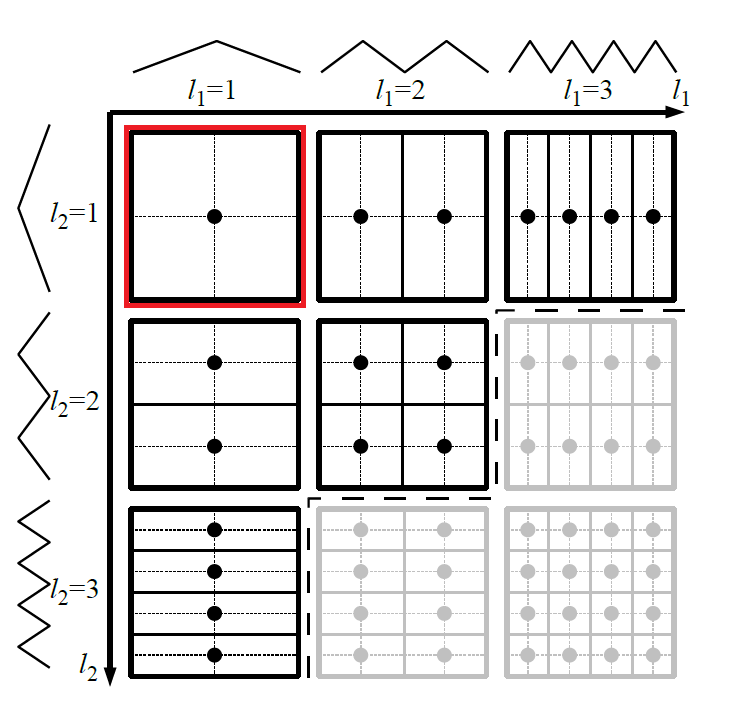
\includegraphics[width=0.30\textwidth]{figures/Gitter02}}
	\subfigure[Dünnes Gitter Level 2]{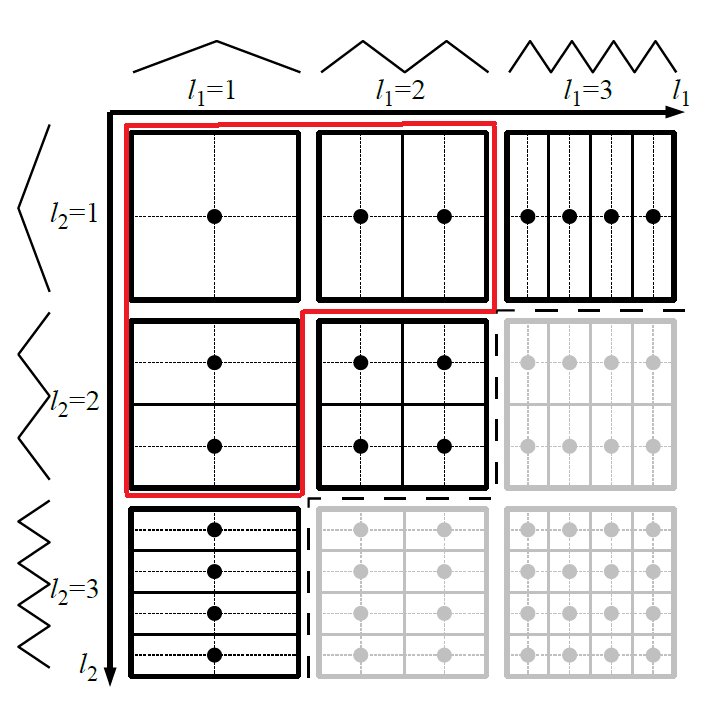
\includegraphics[width=0.30\textwidth]{figures/Gitter05}}
	\subfigure[Dünnes Gitter Level 3]{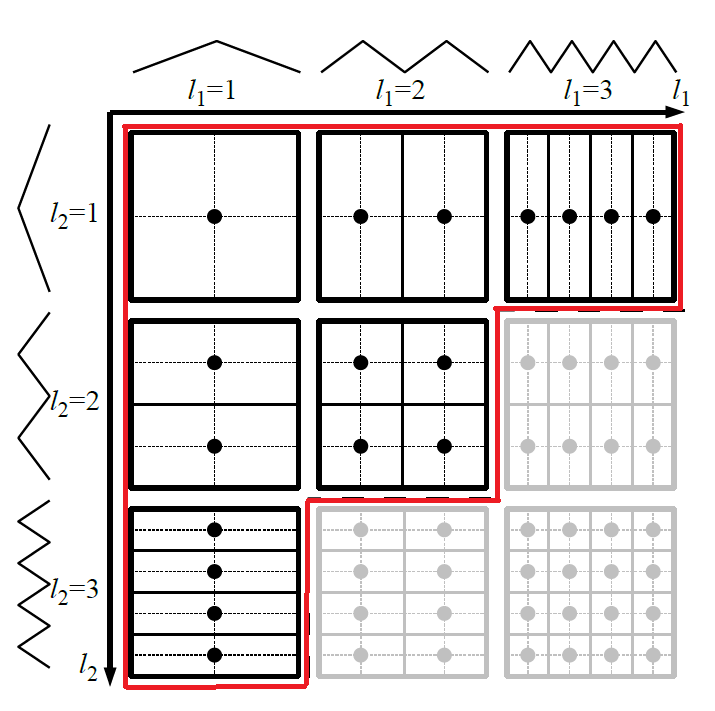
\includegraphics[width=0.30\textwidth]{figures/Gitter06}}
	\caption{Beispiele für zweidimensionale dünne Gitter}
	\label{fig:gitter03}
\end{figure}

In Abbildung \ref{fig:gitter03} ist zu sehen, dass sich im zweidimensionalen Fall bei steigendem Level der Gitter immer eine Diagonale dazukommt. Für den Algorithmus der dünne Gitter Strategie benötigen wir zusätzlich noch ein $S'$ und anstelle von $K$ ein $K'$. Dabei funktioniert $S'$ ganz analog zu $S$ wobei Tupel aus zwei $d$-dimensionalen Vektoren gespeichert werden. Der erste um die Zelle zu beschreiben und der zweite um das Level aus der die korrespondierende Koordinate stammt zu definieren. $K'$ speichert nun die Koordinaten nach Leveln getrennt in verschiedenen Listen oder Arrays und nicht wie $K$ noch alles in einer Liste/Array.

Die Funktionsweise des folgenden Algorithmus leitet sich von mit dünne Gittern einhergehenden Bedingung an die Inkremente ab. Dabei ist zu beachten, dass $|\underline{m}|_1\leq n+d-1$ gilt. Bei konstanter Dimension erhöht sich pro dazukommende Diagonale um das nächste Gitter zu erzeugen jeweils nur $n$ um eins. Das heißt von den Indeces der Inkremente kann sich maximal eines auf ein neues Level erhöhen damit die Bedingung weiterhin erhalten bleibt. Also erarbeiten wir ausgehend von den alten Schüssen  die neuen, indem einzelne Koordinaten um ein Level erhöht werden. Dabei ist zu beachten, dass innerhalb eines neuen Levels es mehrere mögliche Koordinaten gibt. 


\begin{tcolorbox}
	\begin{algorithmic}
		\Function{sparse\_grid\_strat}{$S',K',L$}{$:cell$}
		\If{$K'=\emptyset$}
		\State $K'[0]=\left[\left\lfloor\frac{N}{2}\right\rfloor\right]$
		\State $max\_coord=K'\left[0\right][0]$
		\State $L=0$
		\State $countCoord = 0$
		\State $position = 0$
		\EndIf
		\If{$S'[last\_index][0]=(K'[0][0],\dots,K'[0][0],max\_coord)$}
		\State $min=\left\lceil\frac{K'[L][0]}{2}\right\rceil$
		\State $K'.add([])$
		\For{\textbf{each } $k\in K'[L]$}
		\State $K'[L+1].add(k-min)$
		\State $K'[L+1].add(k+min)$
		\EndFor
		\State $L++$
		\State $max\_coord=K'\left[L\right][last\_index]$
		\State $countCoord = 0$
		\State $position = 0$
		\EndIf
		\If{$S=\emptyset$}
		\State $S'.add((('K[0][0],\dots,K'[0][0]),(0,\dots,0)))$
		\State \Return $(K'[0][0],\dots,K'[0][0])$
		\Else
		\State $out = S'[0]$
		\If{$countCoord=0$}
		\State $out[1][position]++$
		\EndIf
		\State $out[0][position]=K[out[1][position]][countCoord]$
		\State $countCoord++$
		\If{$countCoord=K[position].size()$}
		\State $countCoord=0$
		\State $position++$
		\If{$position=d$}
		\State $position=0$
		\State $S'.delete(0)$
		\EndIf
		\EndIf
		\State $S'.add(out)$
		\State\Return $out[0]$
		\EndIf
		\EndFunction
	\end{algorithmic}
\end{tcolorbox}

Wir werden jetzt nun wieder den Algorithmus in kleinen Teilen näher betrachten und dabei die Funktionsweise und Komplexität genauer beschreiben.

\smallskip
\hrule
\smallskip

\begin{tcolorbox}
	\begin{algorithmic}
		\If{$K'=\emptyset$}
		\State $K'[0]=\left[\left\lfloor\frac{N}{2}\right\rfloor\right]$
		\State $max\_coord=K'\left[0\right][0]$
		\State $L=0$
		\State $countCoord = 0$
		\State $position = 0$
		\EndIf
	\end{algorithmic}
\end{tcolorbox}

Dies beschreibt den Fall der zu Beginn vorliegt. Hier werden die erste Koordinate und ein paar notwendige Variablen initialisiert. Auf die Funktion der Variablen $countCoord$ und $position$ kommen wir noch später genauer zu sprechen. Die Komplexität ist $O(1)$.

\smallskip
\hrule
\smallskip

\begin{tcolorbox}
	\begin{algorithmic}
		\If{$S'[last\_index][0]=(K'[0][0],\dots,K'[0][0],max\_coord)$}
		\State $min=\left\lceil\frac{K'[L][0]}{2}\right\rceil$
		\State $K'.add([])$
		\For{\textbf{each } $k\in K'[L]$}
		\State $K'[L+1].add(k-min)$
		\State $K'[L+1].add(k+min)$
		\EndFor
		\State $L++$
		\State $max\_coord=K'\left[L\right][last\_index]$
		\State $countCoord = 0$
		\State $position = 0$
		\EndIf
	\end{algorithmic}
\end{tcolorbox}

Dieser Abschnitt beschreibt den Fall, dass neue Koordinaten hinzugefügt werden müssen. Dabei ist die später folgende Iteration so aufgebaut, dass der letzte Schuss eines Koordinatensatzes gerade die Form $(K'[0][0],\dots,K'[0][0],max\_coord)$ hat. Da von vorne nach hinten durch die Dimensionen gezählt wird und $max\_coord$ ebenfalls die letzte Koordinate eines Levels ist. Es wird nun wie zuvor bereits erwähnt eine neue Liste/Array erzeugt, die die Koordinaten des neuen Levels enthalten soll. Die Berechnungen unterscheiden sich dabei nicht von denen bei vollen Gittern. Zum Schliss werden noch einmal $countCoord$ und $position$ gesetzt, da diese wie wir noch sehen werden, sich im Laufe verändert haben und nun zurückgesetzt werden müssen.

Der Vergleich im If ist in $O(d)$. Die Schleife hat $\left\lceil\frac{N}{4}\right\rceil$ Durchläufe, da das gerade die Anzahl der Elemente im vorletzten Level ist. Das letzte Level taucht als Schleife nicht mehr auf, da bis dahin bereits alle Punkte des Spielfelds beschossen sind. Also ist die Schleife in $O(N)$. Davon ausgehend, dass $last\_index$ in $O(1)$ realisiert werden kann hat dieser Abschnitt eine gesamte Komplexität von $O(N+d)$.

\smallskip
\hrule
\smallskip

\begin{tcolorbox}
	\begin{algorithmic}
		\If{$S=\emptyset$}
		\State $S'.add((('K[0][0],\dots,K'[0][0]),(0,\dots,0)))$
		\State \Return $(K'[0][0],\dots,K'[0][0])$
		\Else
		\State $out = S'[0]$
		\If{$countCoord=0$}
		\State $out[1][position]++$
		\EndIf
		\State $out[0][position]=K[out[1][position]][countCoord]$
		\State $countCoord++$
		\If{$countCoord=K[position].size()$}
		\State $countCoord=0$
		\State $position++$
		\If{$position=d$}
		\State $position=0$
		\State $S'.delete(0)$
		\EndIf
		\EndIf
		\State $S'.add(out)$
		\State\Return $out[0]$
		\EndIf
	\end{algorithmic}
\end{tcolorbox}

Der If Abschnitt liegt in $O(1)$ ist aber auch nicht weiter relevant, da er nur einmal aufgerufen wird. Der Else Abschnitt hat zunächst ein paar $O(1)$ Zeilen, da es sich nur um Zugriff oder arithmetische Operationen handelt. Die $size()$ Funktion liegt bei maximalem Level in $O(N)$. Die $delete()$ Funktion ist hier $O(1)$, da das erste Element entfernt wird, was in $O(1)$ geht. Somit hat der Else Teil und damit der gesamte Abschnitt eine Komplexität von $O(N)$.


Daraus ergibt sich für den gesamte Algorithmus ein Zeitkomplexität von $O(N+d)$. Der Speicherbedarf ist für $K'$ analog zu $K$ von den vollen Gittern, also $O(N^2)$. Was $S'$ angeht werden hier mehrere Schüsse gespeichert und auch verwendet. Bildlich im Zweidimensionalen gesprochen wird zu jedem Zeitpunkt eine komplette Diagonale an Inkrementen und deren dazugehörige Schüsse gespeichert. Nach \cite{GG08} ist die Größenordnung der Anzahl an Punkten für dünne Gitter $O(2^nn^{d-1})$. Da wir nur eine Diagonale speichern ergibt sich für unsere Menge an Punkten dennoch:

\begin{equation}
2^nn^{d-1}-2^{n-1}(n-1)^{d-1}=2^n\left(n^{d-1}-\frac{(n-1)^{d-1}}{2}\right)\in O(2^nn^{d-1})
\end{equation}

Also haben wir einen Speicherbedarf von $O(N^2+2^nn^{d-1})$, damit $O(2^nn^{d-1})$.


\subsection{Monte-Carlo Strategie}

Ähnlich wie Strategien aus der Diskretisierung durch dünne und volle Gitter gewonnen wurden, kann eine Strategie aus der Monte-Carlo Diskretisierung abgeleitet werden. Dabei stellt die Wahl der Stützstellen, die bei Gittern noch nach Gesetzmäßigkeiten ausgewählt wurden, effektiv die Strategie dar, so dass diese Punkte den Schüssen entsprechen. Da bei Monte-Carlo diese Stützstellen zufällig gewählt werden, tun wir dies auch hier für unsere (erste) Monte-Carlo Strategie. 

\subsection{Quasi-Monte-Carlo Strategie}


% Literaturverzeichnis ------------------------------------------------
\newpage
\bibliographystyle{alphadinLinkLocal}
%\bibliography{literatur} 

\begin{thebibliography}{WB95}
	\providecommand{\url}[1]{\texttt{#1}}
	\expandafter\ifx\csname urlstyle\endcsname\relax
	\providecommand{\doi}[1]{doi: #1}\else
	\providecommand{\doi}{doi: \begingroup \urlstyle{rm}\Url}\fi
	
	\bibitem[WB95]{WB95}
	\textsc{Welch}, G. ; \textsc{Bishop}, G.:
	\newblock An Introduction to the Kalman Filter  / UNC-CH Computer Science.
	\newblock \,Version:\,1995.
	\newblock  \url{http://www.cs.unc.edu/~welch/media/pdf/kalman_intro.pdf}
	(95-041). --
	\newblock Technical Report. --
	\newblock Online--Ressource
	
	\bibitem[M13]{M13}
	\textsc{Mehlbeer}, F.:
	\newblock \textit{Hierarchische Methoden am Beispiel von Schiffe versenken},
	\newblock Bachelorarbeit Nr.25,
	\newblock Universität Stuttgart,
	\newblock 2013
	
	\bibitem[P10]{P10}
	\textsc{Pflüger}, D.:
	\newblock \textit{Spatially Adaptive Sparse Grids for High-Dimensional Problems},
	\newblock Dissertation,,
	\newblock Technische Universität München,
	\newblock 2010
	
	\bibitem[GG08]{GG08}
	\textsc{Gerstner}, T. ; \textsc{Griebel}, M.:
	\newblock \textit{Sparse Grids},
	\newblock From Encyclopedia of Quantitative Finance,
	\newblock Universität Bonn,
	\newblock 2008
	
\end{thebibliography}


%\iffalse
\end{document}
%\fi
